\documentclass[12pt]{scrreprt}
\usepackage[utf8]{inputenc}
\usepackage{graphicx}
\usepackage[affil-it]{authblk}
\usepackage{caption}
\usepackage{subcaption}
\usepackage{multirow}
\usepackage{amsmath}

\addtokomafont{disposition}{\rmfamily}

\title{
    \textbf{
    Predicting Electricity Demand:\\
    Comparing Traditional and Machine Learning Approaches
    }
}

\author{
    {\Large Dimitrije Stankovic}\\
    {\small 5232098}
}
\affil{University of Aberdeen}
\date{August 2024}


\begin{document}

\maketitle

\tableofcontents

\chapter*{Abstract}
Accurate prediction of electricity demand is vital for efficient infrastructure development. This thesis investigates the effectiveness of traditional regression (TR) methods and machine learning (ML) approaches for electricity demand forecasting. Traditional methods, such as Seasonal ARIMA(X) models, are compared against machine learning models, including Long Short-Term Memory (LSTM) and Gated Recurrent Unit (GRU) networks. The models are compared based on efficiency, explainability, and computational expense. Results show that while ML models can perform well in some cases, traditional methods generally offer comparable or better accuracy with lower computational costs and higher explainability. Consequently, the adoption of ML models for long- and short-term load forecasting may not significantly outperform traditional approaches, though they could be beneficial in other forecasting contexts.

\chapter{Introduction}

The accurate prediction of electricity demand is extremely important to the efficient development of any nation’s infrastructure. Long-term load forecasting (LTLF) helps governments and energy suppliers to develop their infrastructure in future years and decades, whereas short-term load forecasting (STLF) assists in scheduling daily and weekly energy production and routing. Various forecasting methods have been attempted in the past \cite{Nti20, Chung22, Gao23}, and many comparisons of methods have been made \cite{Nti20, Gao23, Chung14}, but accuracy must be balanced with efficiency in a practical environment. As such, this thesis will not solely look at forecasting methods that minimise error but also those which optimise for two, more practical concerns.

The biggest problems in implementing machine learning (ML) methods in real-world environments, like government or business concerns, are computational infrastructure and explainability. Computing ML models often requires extensive computational resources, which can lead to extremely long training times without the proper infrastructure, depending on the dataset and model structure. Not only does model training require significant time, but feature selection and hyperparameter tuning algorithms also add to this duration. As a result, ML models are not always feasible or desirable to run, unless the forecaster has access to a cloud solution or an in-house cluster for computation --- both of which are very expensive.

When it comes to recurrent neural networks (RNNs), such as those used in this thesis, the best feature importance rankings are obtained by repeatedly running a trained model with different parameters and searching for optimal results \cite{Zien09, Wojtas20}. This is unrealistic for large and complex models without the expensive infrastructure previously mentioned, since the energy and time required to do so would be rather a lot, especially if there are many features under examination. Despite the models in this thesis being neither large nor complex, producing good and consistent results proved to be a challenge, both in time and computational expense.

Nevertheless, the financial and computational expense involved in running these models is only one piece of the puzzle. Stakeholders do not blindly trust ML approaches to forecasting in decision-making, since these models are ``black boxes'' \cite{Hoepner21}. Black boxes are models where the input-output/feature-prediction relationship are not discernible without significant computation \cite{Zien09, Wojtas20}, which is a big problem when this relationship is the basis for actionable insights used in decision-making \cite{Hoepner21}. Important infrastructure decisions should be informed, and one cannot be fully informed without justifications, such as those provided by explainable models. Given this aversion to black boxes, traditional regression (TR) might be preferred. And given these shortcomings in ML modelling, one might ask whether it is, in fact, worth using ML techniques for numerical forecasting. The intention of this thesis is to answer precisely this question.

\chapter{Data and Hardware}

The data used for this thesis comes from two sources: National Grid Electricity System Operator (ESO) for national demand and solar generation/capacity data (used solely for proxying weather), and the Meteostat API for Python provided weather data. The data from ESO is half-hourly, spanning from Jan 2009 to May 2024, and Meteostat was called to span from 2011 onwards, due to missing data before that time. Values were aggregated at the month level starting in 2011 for LTLF, and at the daily level throughout 2022 for STLF.

As regards the weather data, temperature and windspeed were (simply) averaged between London, Edinburgh, and Cardiff to proxy weather for all of Great Britain. Certain values were missing from Meteostat when pulling daily data, so a linear interpolation was used to fill the missing values. Besides this, and some more programmatic concerns (see supplementary materials), the data was clean. 

The specific columns used from these datasets are the following:
\begin{itemize}
    \item From the ESO dataset:
    \begin{itemize}
        \item[$\circ$] \texttt{SETTLEMENT\_DATE} --- the date at which energy consumption and balancing was settled
        \item[$\circ$] \texttt{SETTLEMENT\_PERIOD} --- the half-hour period at which energy consumption and balancing was settled
        \item[$\circ$] \texttt{ND} --- the national energy demand in megawatts
        \item[$\circ$] \texttt{EMBEDDED\_SOLAR\_GENERATION} --- megawatts generated in the settlement period by local solar sources
        \item[$\circ$] \texttt{EMBEDDED\_SOLAR\_CAPACITY} --- megawatts possible to generate in the settlement period from local solar sources
    \end{itemize}
    \item From the Meteostat API:
    \begin{itemize}
        \item[$\circ$] \texttt{tavg} --- the average temperature in the specified time range
        \item[$\circ$] \texttt{wspd} --- the average wind speed in the specified time range
    \end{itemize}
\end{itemize}

In addition to these columns, three more were created from the data. \texttt{YEAR\_MONTH} and \texttt{YMD} aggregate all values into monthly and daily values by mean, respectively. Since sun duration data was incomplete from Meteostat, \texttt{sun\_eff} was created as a proxy for it:

\[\texttt{sun\_eff}=\frac{\texttt{EMBEDDED\_SOLAR\_GENERATION}}{\texttt{EMBEDDED\_SOLAR\_CAPACITY}}\]

\newpage
The hardware used for this project is the following:
\begin{itemize}
    \item CPU --- AMD Ryzen 5 5600 6-Core (12-Thread) Processor (3.5 GHz)
    \item GPU --- Nvidia RTX 2060 Super (6 GB VRAM)
    \item RAM --- 48 GB DDR4 (2133 MT/s)
\end{itemize}

\chapter{Traditional Regression}

\section{Seasonal AutoRegressive Integrated Moving Average (with eXogenous variables)}

Performing some exploratory data analysis on national demand data shows that the data is extremely seasonal at the year-month level, seen in figure \ref{fig:s_decomp_ltlf} ``Seasonality", with a persistent downward trend, ibid. ``Trend". Predictably, the largest absolute residual (shock) happens in 2020, specifically when the nationwide lockdown was announced as a result of the COVID-19 pandemic. See the lowest trough in subplot ``Residual". It will be interesting to see how each model will perform when presented with such a shock.

\begin{figure}[h]
    \centering
    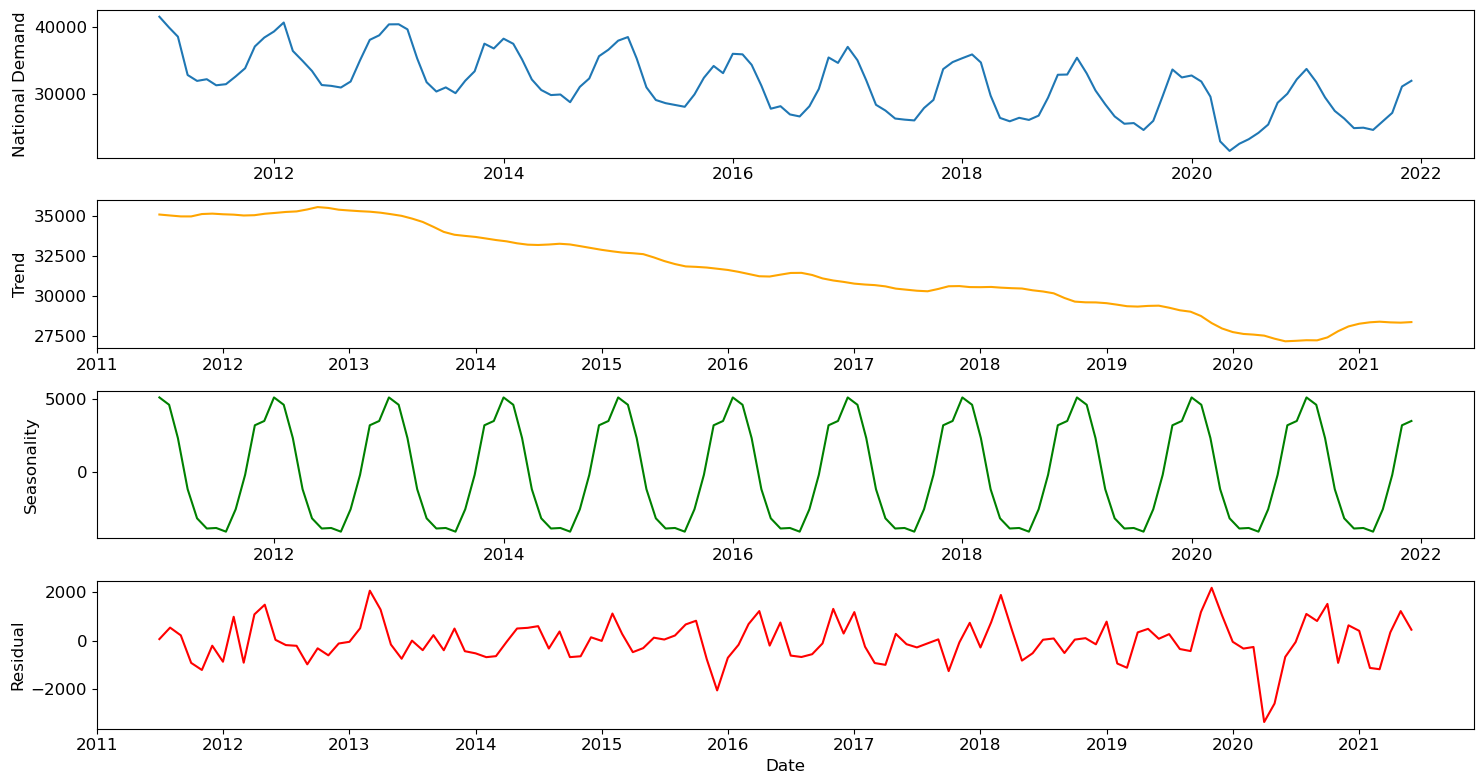
\includegraphics[scale=0.35]{Images/s_decomp_ltlf.png}
    \caption{The seasonal decomposition of mean monthly national demand.}
    \label{fig:s_decomp_ltlf}
\end{figure}

The seasonal decomposition of the mean daily demand data reflects the overall yearly cosine-shaped trend (figure \ref{fig:s_decomp_stlf} ``Trend"), but a shock is observed around Christmas (ibid. ``Residual") --- likely because of the holiday. This shock is also something to look out for when evaluating the models' tracking of the data. Strong weekly seasonality is observed (ibid. ``Seasonality"), with troughs in the weekends.

\begin{figure}[h!]
    \centering
    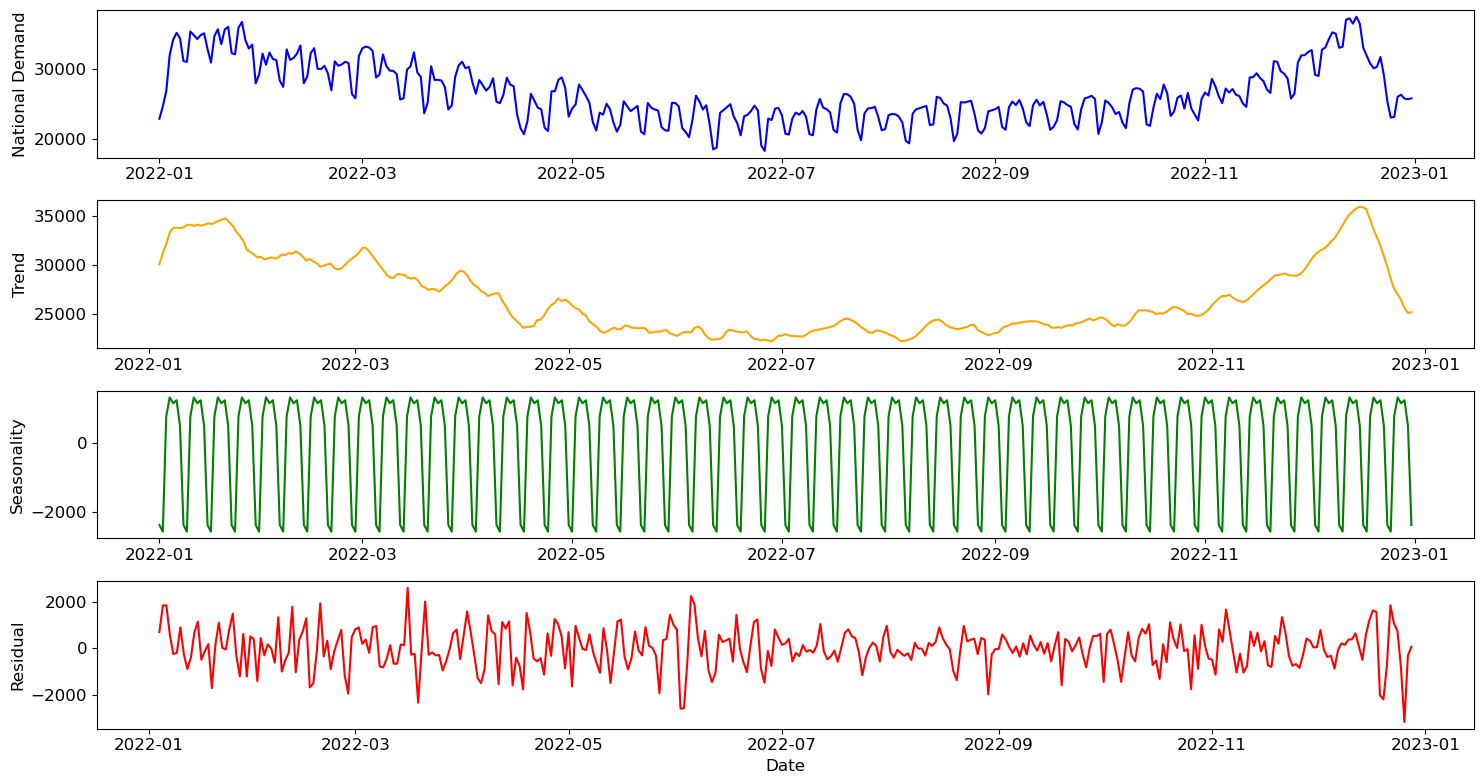
\includegraphics[scale=0.35]{Images/s_decomp_stlf.png}
    \caption{The seasonal decomposition of mean daily national demand.}
    \label{fig:s_decomp_stlf}
\end{figure}

The literature tends to use ARIMA(X)-based models --- AutoRegressive Integrated Moving Average (with eXogenous variables) --- for forecasting energy demand when using a traditional method \cite{Nti20}. A load forecasting model needs to be able to handle seasonality as well as trend, so SARIMA(X) --- Seasonal ARIMA(X) --- is the most common of these. With SARIMAX, instead of supplying only the autoregressive, differencing, and moving average terms, $(p,d,q)$, that one normally would in ARIMA, an extra parametrisation is supplied to specify the seasonal order of the time series, $s$, and the seasonally lagged terms of the regression, $(P,D,Q)$. The full mathematical specification of a SARIMAX model is the following \cite{Korstanje21}:

\begin{equation}
    y_t = \sum_{i=1}^{N}[\beta_{it} x_{it}] + u_{it}
\end{equation}

\begin{equation}
    \phi_p(L) \tilde{\phi}_P(L^s) \Delta_d \Delta_D u_t = A(t) + \theta_q(L) \tilde{\theta}_Q(L^s) \zeta_t
\end{equation}
where equation 3.1 covers the contribution of the exogenous variables $x_i, ..., x_N$ and the error term $u_{it}$ in $y_t$, and the equation 3.2 covers the contribution of the lags to future values of the time series. A quick breakdown of the terms in equation 3.2 follows:

\begin{itemize}
    \item $\phi_p(L)$ and $\tilde{\phi}_P(L^s)$ are the AR and seasonal AR components of the model on the lag operators $L$ and $L^s$
    \item $\Delta_d$ and $\Delta_D$ are the non-seasonal and seasonal integration (differencing) orders
    \item $\theta_q(L)$ and $\tilde{\theta}_Q(L^s)$ are the MA and seasonal MA components of the model on the lag operators $L$ and $L^s$
    \item $\zeta_t$ is the residual of the MA component
    \item and $u_t$ comes from the first equation
\end{itemize}

These equations are fit to the data using maximum likelihood estimation (MLE), the explanation of which is beyond the scope of this thesis, making the resulting model deterministic. When discussing a model with orders $(p,d,q)$ and $(P,D,Q,s)$, the convention is to write: $\textrm{SARIMA } (p,d,q)\times(P,D,Q,s)$ or $\textrm{SARIMAX } (p,d,q)\times(P,D,Q,s)$

The first model construction, a SARIMA for LTLF, will be done by hand in order to demonstrate the clarity of the process (as compared later with ML model construction). The first step is to check for stationarity. This can be done in a few different ways, but the most common is the augmented Dickey-Fuller test, which simply gives a $p$-value under the null hypothesis that the series is non-stationary. For this model, it is only necessary to test \texttt{ND} at the year-month level. After a single differencing, the series was stationary, so $d$ and $D$ should be 1.

The next step is to find the AR and MA orders. This can be done by looking at the autocorrelation function (ACF) and the partial ACF (PACF), which describe the significance of the lags of the time series. The difference between them is that, for lags earlier than $y_{t-1}$, the PACF removes the effects of intervening lags on $y_t$. So, while the ACF will include the effect of $y_{t-1}, y_{t-2}, ..., y_{t-k}$ in determining whether lag $k$ is significant, the PACF only accounts for the effect of $y_{t-k}$ on $y_t$. All this to say, to select the AR component (which considers the lagged \textit{values} of a time series), choose the lag $p$ after which the PACF shows no significant direct correlation between $y_t$ and $y_{t-(p+1)}$. And since the MA component considers the \textit{residuals} of a time series, the same is done in the ACF to select $q$. Then look at the recurring peaks to determine seasonality, $s$, and the seasonally lagged $P$ and $Q$. Theoretically, one should determine $p+1$ by checking where the first lag is in the shaded blue area (the confidence interval under the null hypothesis that the lags are not significant), but the common advice is to use only \textit{clearly} significant lags.

\begin{figure}[h]
    \centering
    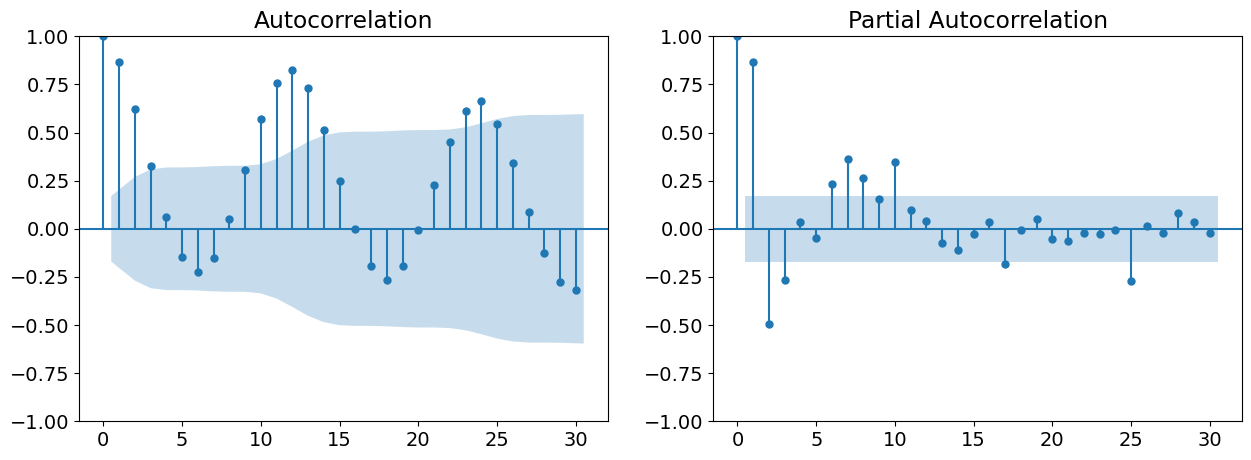
\includegraphics[scale=0.5]{Images/ltts_acf.png}
    \caption{The ACF and PACF of mean monthly national demand.}
    \label{fig:ltts_acf}
\end{figure}

Following the outlined steps, the resultant model is: $\textrm{SARIMA }(1,1,2)\times(1,1,2,12)$.

This way of specifying the model is fine, but there is a more rigorous way to do it: grid search. The method begins with choosing the maximum parameters using the method defined earlier, but making sure it is the theoretical lag (where the next lag is within the shaded area) and choosing a model selection criterion to optimise. Then take the ranges up to and including these maximum values and make a Cartesian product (every possible combination of the ranges) to generate the model specifications to try, selecting only the optimal model in terms of the selection criterion.

The Aikake Information Criterion (AIC) was chosen as the model selection criterion for the SARIMA(X) models. It is defined as:
\[\textrm{AIC} = 2k - 2\textrm{ln}(\hat{L})\]
where $k$ is the number of features or lags in the model and $\hat{L}$ is the maximum of the likelihood function (basically a goodness-of-fit metric). A lower AIC is better, meaning the criterion punishes models with too many features (as there is a risk of overfitting) and rewards models with high goodness-of-fit (to balance against underfitting). So, AIC is a sound way to select well-fitting models while making sure that the features used contribute ``enough" information to the model. That said, standard metrics are also examined to evaluate the performance of a model, viz. root mean squared error (RMSE) and mean average percentage error (MAPE):

\begin{equation}
    \begin{split}
        \text{RMSE} &= \sqrt{\frac{1}{n} \sum_{i=1}^{n} (y_i - \hat{y}_i)^2} \\
        \text{MAPE} &= \frac{100}{n} \sum_{i=1}^{n} \left| \frac{y_i - \hat{y}_i}{y_i} \right|
    \end{split}
\end{equation}
where:
\begin{itemize}
    \item $y_i$ is the actual value
    \item $\hat{y}_i$ is the predicted value
    \item $n$ is the number of observations
\end{itemize}

The generated LTLF SARIMA model is: $\textrm{SARIMA }(0,1,1)\times(0,1,1,12)$.
Then the \texttt{sun\_eff} proxy and weather data from the Meteostat API are added, generating the optimal long-term SARIMAX model: $\textrm{SARIMAX }(0,1,1)\times(0,1,2,12)$.
The same is then done for the short-term (daily) data over 2022, yielding the following STLF models: $\textrm{SARIMA }(0,1,4)\times(0,1,4,7)$ and $\textrm{SARIMAX }(0,1,4)\times(0,1,4,7)$.

\newpage

\section{Results}

The plots below include a shaded area for the confidence interval of the predicted values for the reader's convenience. Training data extends from 2011-2022, but for readability, the plot was truncated. STLF plots were also truncated in the same way.

\begin{figure}[h!]
    \centering
    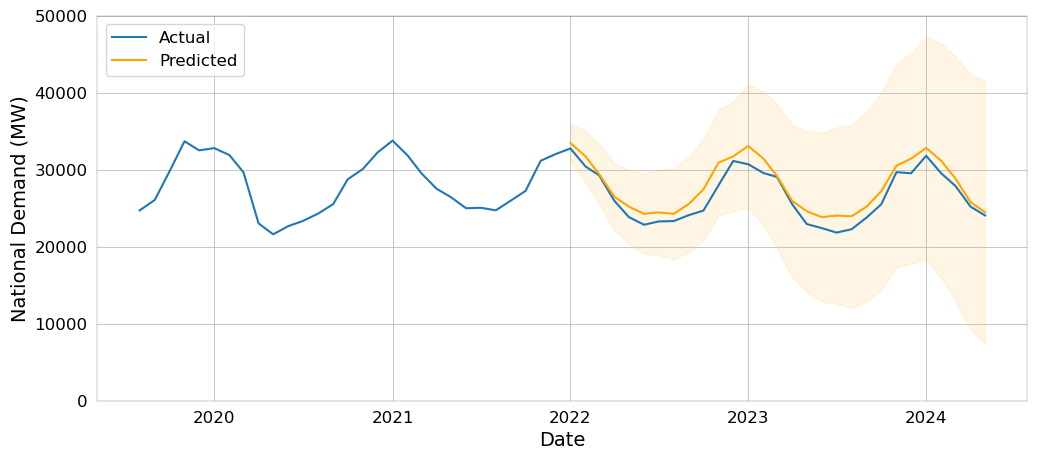
\includegraphics[scale=0.5]{Images/ltts_of_fcast.png}
    \caption{The manually constructed LTLF SARIMA forecast for mean monthly demand.}
    \label{fig:ltts_of_fcast}
\end{figure}

\begin{figure}[h!]
    \centering
    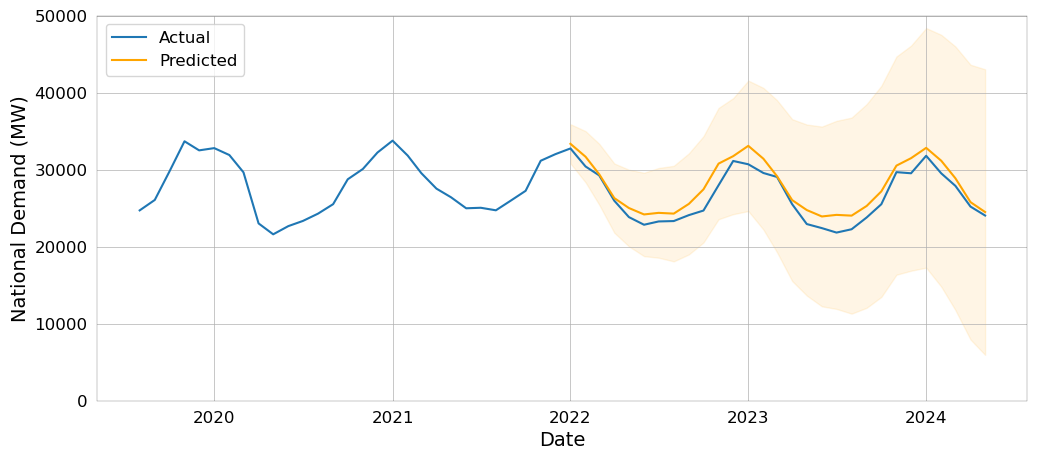
\includegraphics[scale=0.5]{Images/ltts_grid_fcast.png}
    \caption{The LTLF SARIMA forecast for mean monthly demand.}
    \label{fig:ltts_grid_fcast}
\end{figure}

The first comparison to make, is between the manually constructed (figure \ref{fig:ltts_of_fcast}) and the grid optimised (figure \ref{fig:ltts_grid_fcast}) LTLF SARIMA models. The reason for the manually constructed model is to show that near-optimal results are attainable without hyperparameter tuning (like grid search). This is not the case for the ML models examined in section 4. Looking at the plots alone, it seems that these SARIMA models perform identically, and table 3.1 will show that they essentially do.

\begin{figure}[h!]
    \centering
    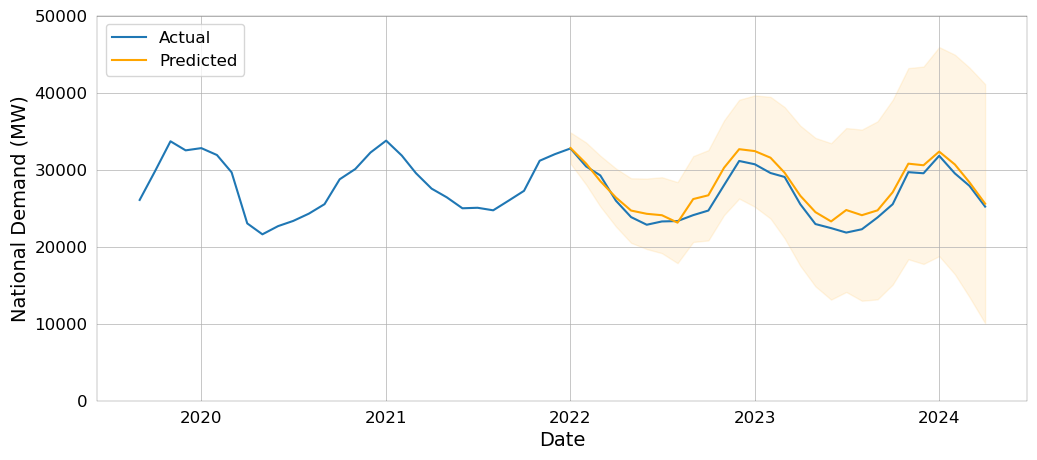
\includegraphics[scale=0.5]{Images/ltex_fcast.png}
    \caption{The LTLF SARIMAX forecast for mean monthly demand.}
    \label{fig:ltex_fcast}
\end{figure}

The improvement in figure \ref{fig:ltex_fcast} is subtle, but visible at the jagged trough in the middle of 2022 and the jagged peak at the end of 2023. This is because the added information from the exogenous variables allows for better tracking.

\begin{figure}[h!]
    \centering
    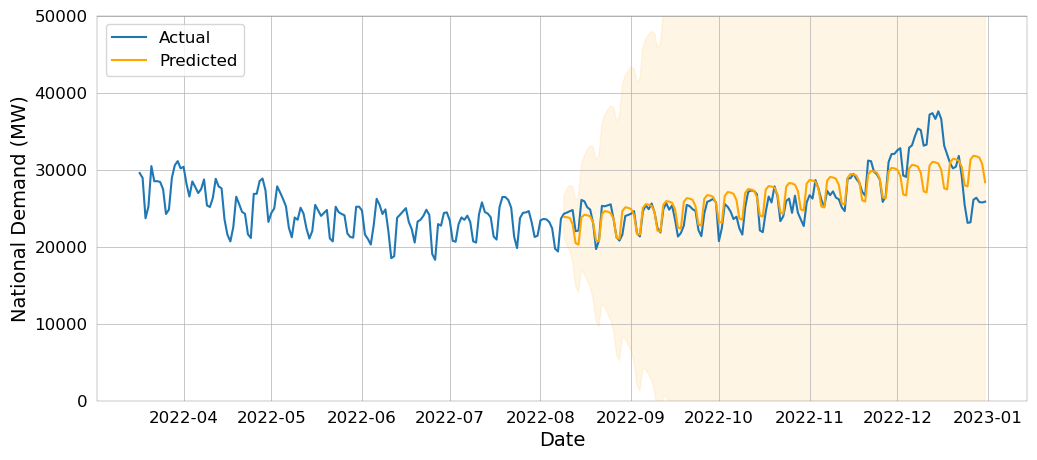
\includegraphics[scale=0.5]{Images/stts_fcast.png}
    \caption{The short-term SARIMA forecast for mean daily demand.}
    \label{fig:stts_fcast}
\end{figure}

\begin{figure}[h!]
    \centering
    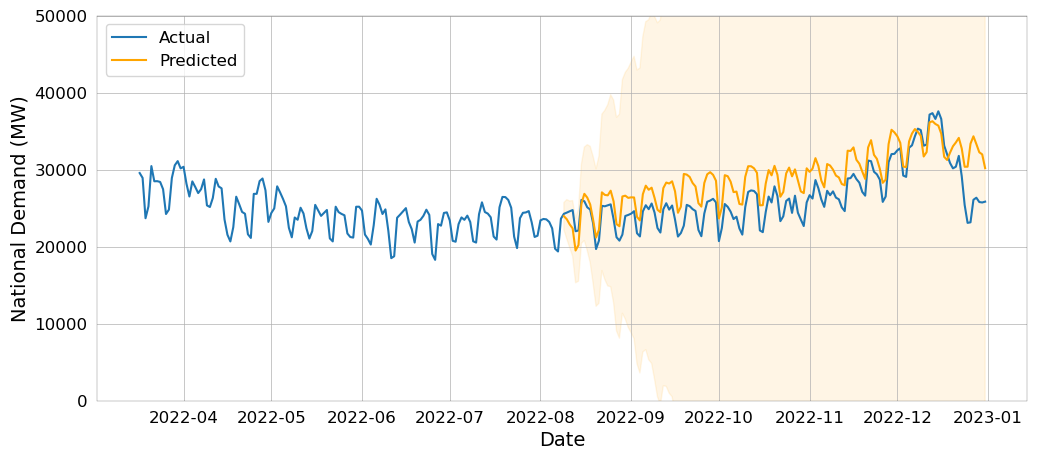
\includegraphics[scale=0.5]{Images/stex_fcast.png}
    \caption{The short-term SARIMAX forecast for mean daily demand.}
    \label{fig:stex_fcast}
\end{figure}

The differences between these models are fairly obvious: the tracking is much better in figure \ref{fig:stex_fcast} than in figure \ref{fig:stts_fcast}, which is the same phenomenon as in the LTLF SARIMAX compared to its SARIMA counterparts. The problem in this model is the chronic overestimation of the test data. This is likely due to the noise that is introduced by the added variables' residuals.

\begin{table}[h!]
    \centering
    \begin{tabular}[h!]{|c|c c c|}
        \hline
        Model & AIC & RMSE & MAPE \\
        \hline
        LTLF SARIMA (manual) & 2071.03 & 1478.63 & 5.00\%\\
        \hline
        LTLF SARIMA & 2064.83 & 1482.50 & 5.01\%\\
        \hline
        LTLF SARIMAX & 2014.24 & 1350.72 & 4.50\%\\
        \hline
        STLF SARIMA & 3706.77 & 2480.77 & 6.34\%\\
        \hline
        STLF SARIMAX & 3525.65 & 3207.76 & 11.16\%\\
        \hline
    \end{tabular}
    \caption{Forecast metrics for all TR models.}
    \label{tab:tr_metrics}
\end{table}

Comparing the manual and automated LTLF SARIMA models, it is clear that the four extra lags did not add much to the model, only decreasing the MAPE by 0.01\%, as reflected by the reduction in AIC. This is interesting, if only for the fact that the grid search ignores any AR component to the model. Regardless, when adding exogenous variables, the MAPE is decreased by ~0.5\%. On the STLF side of things, SARIMA performs significantly better than SARIMAX. There is something to be said for the improved tracking in STLF SARIMAX, however, and it cannot be overlooked that with more training data, the overestimation problem may be solved.

\chapter{Machine Learning}

\section{Long Short-Term Memory (LSTM) and Gated Recurrent Unit (GRU) Models}

Selection of a single ML method for this task is much more complicated than selecting a TR method. Many different models are capable of numerical forecasting \cite{Gao23}, but the most logical kind to use in time-series forecasting are Recurrent Neural Networks (RNNs). A simple RNN is shown in figure \ref{fig:rnn}.

\begin{figure}[h!]
    \centering
    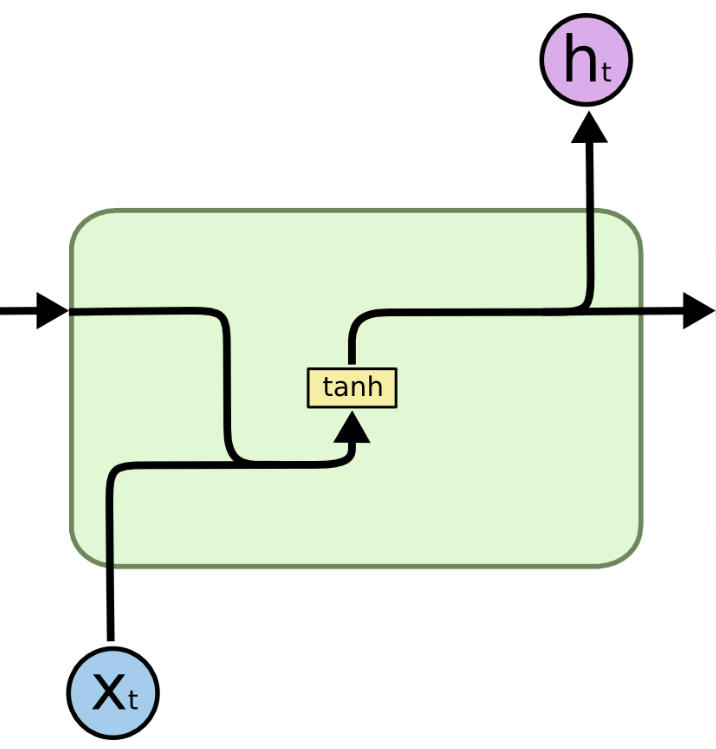
\includegraphics[scale=0.65]{Images/rnn.png}
    \caption{Diagram for a simple RNN \cite{Olah15}}
    \label{fig:rnn}
\end{figure}

The equation that defines this cell structure is:

\begin{equation}
    h_t = \tanh(W \cdot [h_{t-1}, x_t])
\end{equation}
where:
\begin{itemize}
    \item $h_t$ is the hidden state at time $t$
    \item $x_t$ is the input vector at time $t$
    \item $W$ is the weight matrix applied to the concatenation of $h_{t-1}$ and $x_t$
    \item $\tanh$ is the hyperbolic tangent activation function
\end{itemize}

Simple RNNs are not very complex or, consequently, very efficient at prediction as compared to more complex variations of the model. They suffer from the `vanishing gradient problem', which means that RNNs have trouble deciding what information to keep and what to discard. Long short-term memory (LSTM) models were introduced to fix this problem and have been very successful \cite{Nti20, Chung22, Olah15}. LSTMs are mainly used in the field of natural language processing \cite{Olah15, Yin17}, but their applications to numerical forecasting --- particularly in energy demand prediction --- have been quite successful \cite{Nti20, Chung22}.

\begin{figure}[h!]
    \centering
    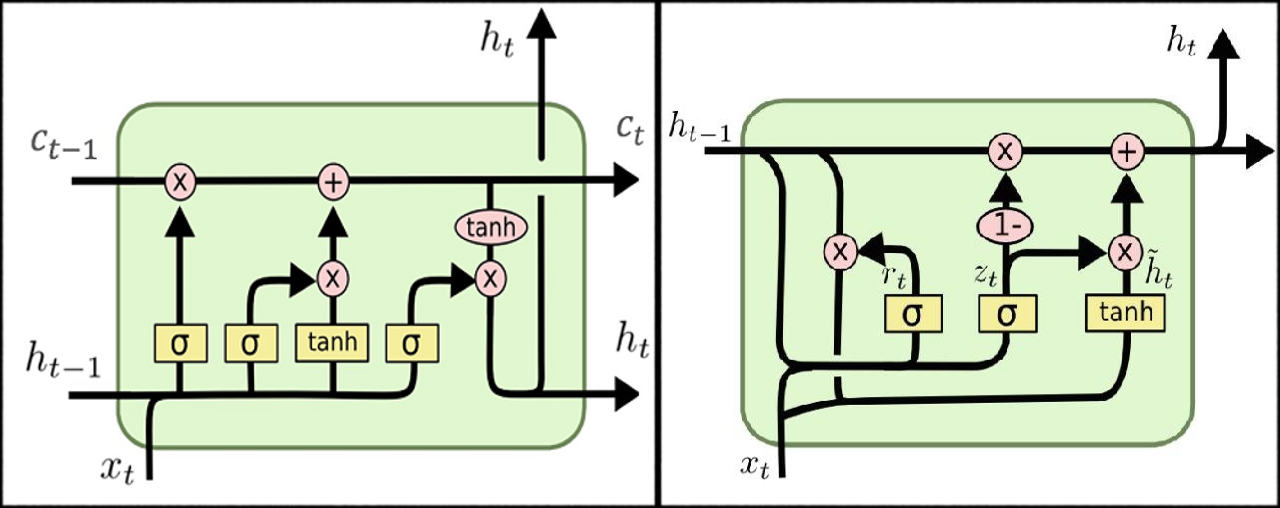
\includegraphics[scale=0.8]{Images/lstm_gru.png}
    \caption{Diagrams for LSTM unit (left) and GRU unit (right) \cite{Olah15}}
    \label{fig:lstm_gru}
\end{figure}

The LSTM cell structure can be expressed with the equations:
\begin{align}
    \begin{split}
        f_t &= \sigma(W_f \cdot [h_{t-1}, x_t] + b_f) \\
        i_t &= \sigma(W_i \cdot [h_{t-1}, x_t] + b_i) \\
        \tilde{C}_t &= \tanh(W_C \cdot [h_{t-1}, x_t] + b_C) \\
        C_t &= f_t \ast C_{t-1} + i_t \ast \tilde{C}_t \\
        o_t &= \sigma(W_o \cdot [h_{t-1}, x_t] + b_o) \\
        h_t &= o_t \ast \tanh(C_t)\\
    \end{split}
\end{align}
where:
\begin{itemize}
    \item $f_t$ is the forget gate activation vector.
    \item $i_t$ is the input gate activation vector.
    \item $\tilde{C}_t$ is the candidate cell state.
    \item $C_t$ is the updated cell state.
    \item $o_t$ is the output gate activation vector.
    \item $W_f, W_i, W_C, W_o$ are the weight matrices for each gate.
    \item $b_f, b_i, b_C, b_o$ are the bias terms for each gate.
    \item $\sigma$ is the sigmoid activation function.
    \item $\ast$ is element-wise multiplication.
\end{itemize}

This is a lot of information to put in one cell, especially a cell that will be recurrently trained, but LSTMs tend to be extremely good in use cases where RNNs suffer from vanishing gradients \cite{Olah15}. A much newer class of models, gated recurrent unit (GRU) models, achieve comparable results in the same use cases \cite{Chung14, Yin17, Nti20}, while simplifying the cell structure drastically (see figure \ref{fig:lstm_gru}).

The equations that define the GRU cell structure are:
\begin{align}
    \begin{split}
        z_t &= \sigma(W_z \cdot [h_{t-1}, x_t]) \\
        r_t &= \sigma(W_r \cdot [h_{t-1}, x_t]) \\
        \tilde{h}_t &= \tanh(W \cdot [r_t \ast h_{t-1}, x_t]) \\
        h_t &= (1 - z_t) \ast h_{t-1} + z_t \ast \tilde{h}_t \\
    \end{split}
\end{align}
where:
\begin{itemize}
    \item $z_t$ is the update gate activation vector.
    \item $r_t$ is the reset gate activation vector.
    \item $\tilde{h}_t$ is the candidate hidden state.
    \item $W_z, W_r, W$ are the weight matrices for the gates and candidate activation.
\end{itemize}

Essentially, GRU cells reduce the input and forget gates to a simpler update gate. This allows for much less computational expense, which is impressive considering that there has been no clear indication in the literature that one is `better' than the other for numerical forecasting in all cases \cite{Korstanje21, Yin17, Olah15}.

TensorFlow and the Keras API were used when training and testing these ML models. The precise implementation of the models will be left to the supplementary materials, but the parameters chosen are the same as those for datasets of comparable size in the literature \cite{Korstanje21, Hogg101, Hogg102}. No hyperparameter tuning was conducted due to a lack of computational resources or access to such resources (see section 2). As in section 3, mean monthly/daily national demand is the predicted variable, with models that predict based on time series data alone (LTLF/STLF) and those that use exogenous variables as well (LTLF-X/STLF-X). All four forecasts were conducted (with the same parameters) using both LSTM and GRU, totalling 8 models.

Training, validation, and test sets were taken from the data as follows: 
\begin{table}[h]
    \centering
    \begin{tabular}{|l|c c c|}
        \hline
        Forecast & Training & Validation & Test  \\
        \hline
        LTLF & 2009-01--2016-12 & 2017-01--2019-12 & 2020-01--2024-05 \\
        \hline
        LTLF-X & 2011-01--2016-12 & 2017-01--2019-12 & 2020-01--2024-05 \\
        \hline
        STLF(-X) & 2022-01-01--2022-04-30 & 2022-05-01--2022-06-30 & 2022-07-01--2022-12-31\\
        \hline
    \end{tabular}
    \caption{Caption}
    \label{tab:train_val_test}
\end{table}

As mentioned in section 2, there is missing weather data for the period before 2011, so those dates cannot be used to train the LTLF-X models. This difference will be reflected in the results.

\newpage

\section{Results}

The results of these models are very hard to discuss with any certainty. Unlike TR models like SARIMAX, the models are not deterministic, so each time the model is trained, there is a different fit. This makes comparing ML and TR models very cumbersome, since there is added noise to every training of every model with every set of parameters. More consistency could be achieved with hyperparameter tuning \cite{Gao23}, but the nature of training neural networks makes for very unpredictable results. There is randomness in the initialisation of weights, the model is optimised using gradient descent on a non-convex surface/hypersurface (resulting in many possible local minima/maxima), and there is noise in the data, all of which lead to an unpredictable and non-normally distributed set of results and metrics. Because the metrics are not normally distributed (or likewise meet the requirements for statistical testing), extracting confidence intervals is also impossible. That said, the best one can do is to average the resultant metrics. In this case, each model was run 30 times and an average of each metric is calculated afterwards, which is shown in table \ref{tab:ml_metrics}. The only new metric used for ML models is the $\textrm{R}^2$ coefficient:

\begin{equation}
    R^2 = 1 - \frac{\sum_{i=1}^{n} (y_i - \hat{y}_i)^2}{\sum_{i=1}^{n} (y_i - \bar{y})^2}
\end{equation}
with the same terms as in Equation 3.3.

\begin{table}[h]
    \centering
    \begin{tabular}{|l | c c c c|}
        \hline
        Forecast & Model & MAPE & RMSE & $\textrm{R}^2$\\ 
        \hline
        \multirow{2}{*}{LTLF} & LSTM & 9.80 & 3030 & 0.082 \\
                              & GRU  & 9.48 & 2899 & 0.212 \\ 
        \hline
        \multirow{2}{*}{STLF} & LSTM & 9.60 & 3347 & 0.202 \\
                              & GRU  & 6.21 & 2039 & 0.684 \\ 
        \hline
        \multirow{2}{*}{LTLF-X} & LSTM & 7.82 & 2354 & 0.493 \\
                                & GRU  & 7.49 & 2258 & 0.540 \\ 
        \hline
        \multirow{2}{*}{STLF-X} & LSTM & 7.73 & 2531 & 0.562 \\
                                & GRU  & 7.98 & 2591 & 0.538 \\ 
        \hline
    \end{tabular}
    \caption{A comparison of key metrics from the ML models.}
    \label{tab:ml_metrics}
\end{table}

Figure \ref{fig:ltlf_ml} demonstrates that GRU performs somewhat better than LSTM at LTLF, but the difference is not stark unless consulting table \ref{tab:ml_metrics} for the $\textrm{R}^2$ values. The way to see that GRU is doing slightly better is to look at the smoothness of the prediction plot compared to LSTM at the beginning of 2021. Interpreting this is difficult, but it seems to be related to the tracking ability of the model, which will be apparent in the STLF models. Figure \ref{fig:ltlfx_ml} shows models that perform almost identically, which corroborates table \ref{tab:ml_metrics}.

\begin{figure}[b!]
    \centering
    \begin{subfigure}{.5\textwidth}
        \centering
        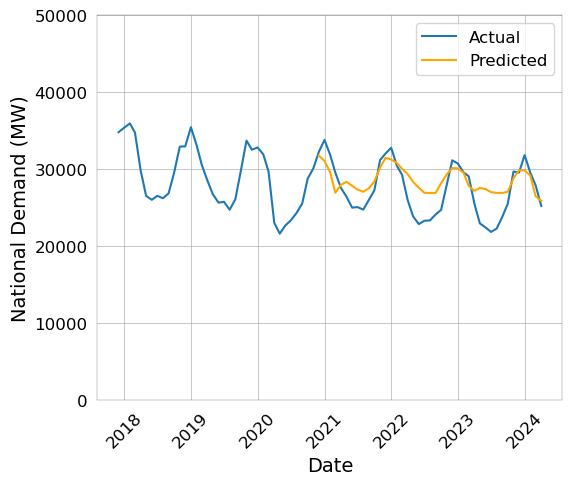
\includegraphics[width=\linewidth]{Images/ltoc_plot.png}
        \caption{LSTM}
        \label{fig:ltoc_plot}
    \end{subfigure}%
    \begin{subfigure}{.5\textwidth}
        \centering
        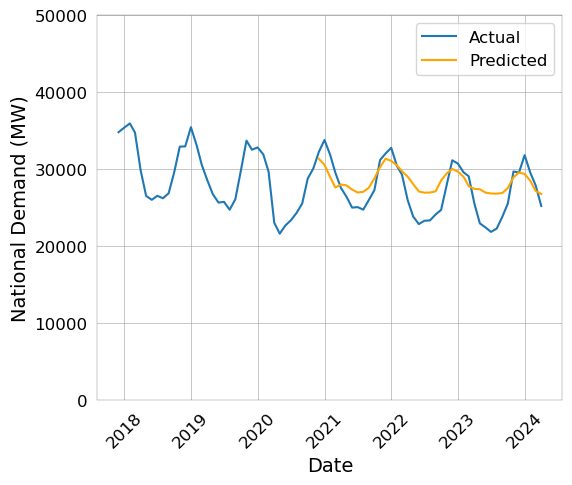
\includegraphics[width=\linewidth]{Images/gltoc_plot.png}
        \caption{GRU}
        \label{fig:gltoc_plot}
    \end{subfigure}
    \caption{LTLF ML models.}
    \label{fig:ltlf_ml}
\end{figure}

\begin{figure}[b!]
    \centering
    \begin{subfigure}{.5\textwidth}
        \centering
        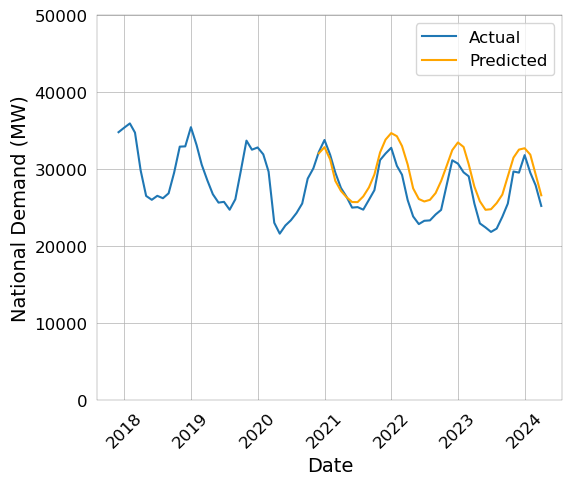
\includegraphics[width=\linewidth]{Images/ltmc_plot.png}
        \caption{LSTM}
        \label{fig:ltmc_plot}
    \end{subfigure}%
    \begin{subfigure}{.5\textwidth}
        \centering
        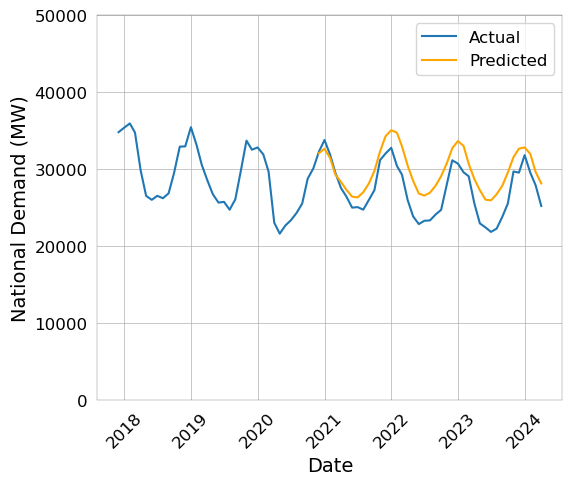
\includegraphics[width=\linewidth]{Images/gltmc_plot.png}
        \caption{GRU}
        \label{fig:gltmc_plot}
    \end{subfigure}
    \caption{LTLF-X ML models.}
    \label{fig:ltlfx_ml}
\end{figure}

As for STLF, GRU stands out as very obviously better. The tracking is very good at all points throughout the test set, especially compared with the LSTM STLF model. The model is constructed in the exact same way, so this result is very surprising, but reflected in the average of 30. This superiority is not evident in the STLF-X GRU, where both models perform about the same -- LSTM underestimating, but GRU overestimating.

\begin{figure}[t!]
    \centering
    \begin{subfigure}{.5\textwidth}
        \centering
        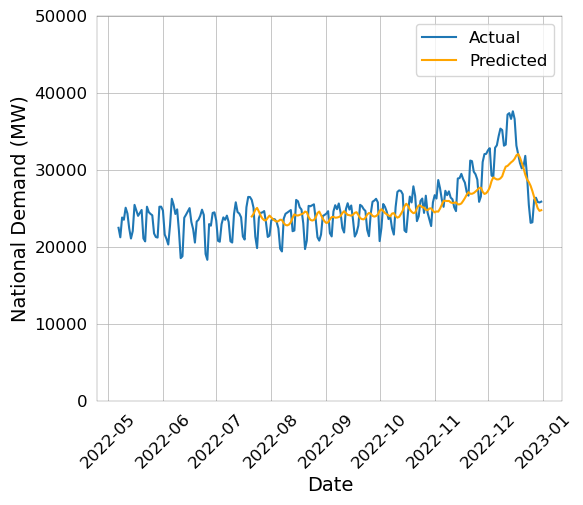
\includegraphics[width=\linewidth]{Images/stoc_plot.png}
        \caption{LSTM}
        \label{fig:stoc_plot}
    \end{subfigure}%
    \begin{subfigure}{.5\textwidth}
        \centering
        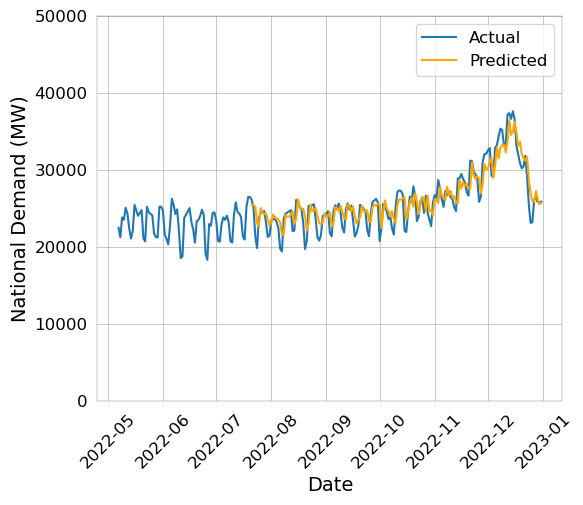
\includegraphics[width=\linewidth]{Images/gstoc_plot.png}
        \caption{GRU}
        \label{fig:gstoc_plot}
    \end{subfigure}
    \caption{STLF ML models.}
    \label{fig:stlf_ml}
\end{figure}

\begin{figure}[h]
    \centering
    \begin{subfigure}{.5\textwidth}
        \centering
        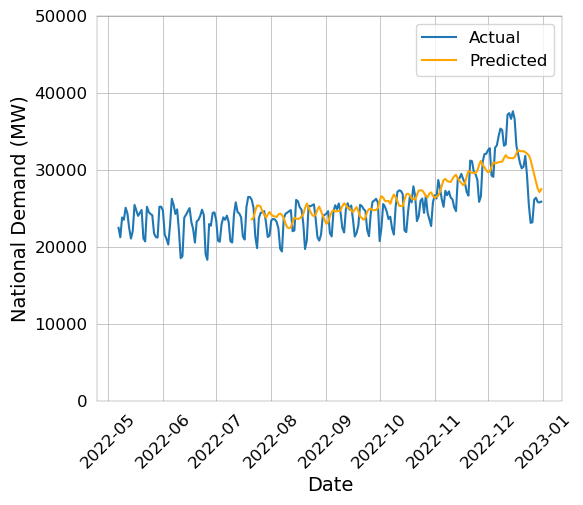
\includegraphics[width=\linewidth]{Images/stmc_plot.png}
        \caption{LSTM}
        \label{fig:stmc_plot}
    \end{subfigure}%
    \begin{subfigure}{.5\textwidth}
        \centering
        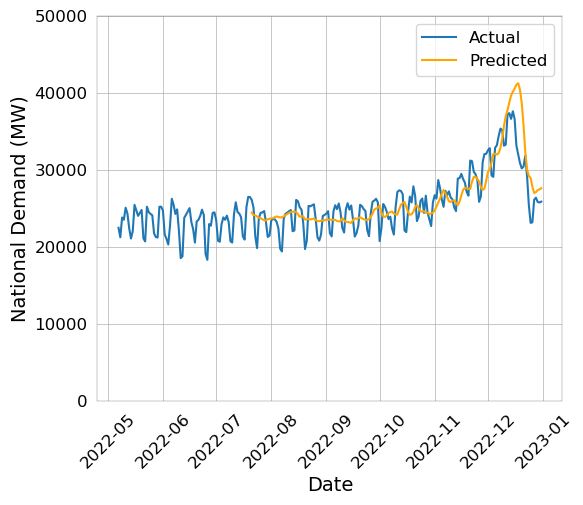
\includegraphics[width=\linewidth]{Images/gstmc_plot.png}
        \caption{GRU}
        \label{fig:gstmc_plot}
    \end{subfigure}
    \caption{STLF-X ML models.}
    \label{fig:stlfx_ml}
\end{figure}

\newpage

As is evident in figure \ref{tab:ml_metrics} and the plots below, there is no evidence to support that either LSTM or GRU performs better at load forecasting as a whole. This is already known from the literature \cite{Chung14}. However, there is one outlying use case, and that is STLF: GRU is significantly better at tracking short-term time series without exogenous variables

\chapter{Comparison and Discussion}

Now that the results from both the TR and ML load forecasting models have been explained, it is time to answer the question of whether ML methods are worth pursuing in energy demand forecasting. As a reminder, the criteria that stakeholders generally look for are: high efficiency, high explainability, and low computational expense. Naturally, TR models will have much higher explainability than ML models, unless computational expense is sacrificed in order to run a PFI or SHAP. TR models will also cost less, computationally speaking, since they use simpler calculations to predict values. So, the question becomes: are ML models more efficient than TR models?

\begin{table}[h]
    \centering
    \begin{tabular}{|c | l c c | c c|}
        \hline
        Forecast & Model (ML) & MAPE (ML) & RMSE (ML) & MAPE (TR) & RMSE (TR)\\
        \hline
        \multirow{2}{*}{LTLF} & LSTM & 9.80\% & 3030 & \multirow{2}{*}{5.00\%} & \multirow{2}{*}{1478.63} \\
                              & GRU  & 9.48\% & 2899 & & \\
        \hline
        \multirow{2}{*}{LTLF-X} & LSTM & 7.82\% & 2354 & \multirow{2}{*}{4.50\%} & \multirow{2}{*}{1350.72} \\
                                & GRU  & 7.49\% & 2258 & & \\
        \hline
        \multirow{2}{*}{STLF} & LSTM & 9.60\% & 3347 & \multirow{2}{*}{6.34\%} & \multirow{2}{*}{2480.77} \\
                              & GRU  & 6.21\% & 2039 & & \\
        \hline
        \multirow{2}{*}{STLF-X} & LSTM & 7.73\% & 2531 & \multirow{2}{*}{11.16\%} & \multirow{2}{*}{3207.76} \\
                                & GRU  & 7.98\% & 2591 & & \\
        \hline
    \end{tabular}
    \caption{Combined comparison of key metrics for ML and TR models.}
    \label{tab:all_metrics}
\end{table}

Table \ref{tab:all_metrics} shows that ML models are not better than TR models on their own. The exception to this is STLF-X applications of the ML models, which are both highly efficient. All other ML metrics are either not clearly different from TR metrics, or worse than them. The MAPEs and RMSEs found here seem to be very close to those in literature \cite{Nti20, Gao23, Chung22}, affirming the conclusions drawn here about performance. 

There are some ways to improve the performance of ML models, i.e. hyperparameter tuning \cite{Gao23}, hybridising models \cite{Chung22}, or providing more historical data, but these techniques would also improve results when applied to TR models. In fact, the grid search that was conducted for the SARIMA(X) models in section 3 is a kind of hyperparameter tuning. Despite this optimisation increasing computational expense, the idea was really to save time selecting parameters manually (as done on page 7, resulting in figure \ref{fig:ltts_of_fcast}) and to prevent overfitting (higher AIC). The highest number of passes needed for a grid search to optimise a TR model in this thesis was 25.

On the other hand, just getting MAPEs out of the ML models required training and running all eight models 30 times. Hypothetically, if one were to have chosen a single model, GRU or LSTM, and then conducted the same process as in the TR forecasting, it would amount to: four models, 30 times, at 50 epochs each, which is \textbf{6,000} full passes of the training data --- forwards and backwards --- through a deep learning algorithm. This is not taking into account the increase in computational expense introduced by larger layer sizes.

Load forecasting in the long- or short-term simply does not seem to be improved by using ML models over TR models. Governments and energy suppliers might find benefit in ML models at other timeframes (or specifically STLF-X with GRU), like ultra-short-term load forecasting \cite{Gao23}, but TR models perform indistinguishably from --- or better than --- ML models in most S/LTLF tasks. Adding to this the general stakeholder desire for explainability, these results do not support the use of these ML models without the proper infrastructure for running complex deep learning models.

\bibliographystyle{ieeetr}
\bibliography{ref}

\end{document}